\documentclass[tikz,border=2pt]{standalone}
% Estilo común de figuras y animaciones (mismos colores que la presentación)
% Compilar con XeLaTeX o LuaLaTeX (fuente TeX Gyre Heros); con pdfLaTeX usa Latin Modern Sans.
\usepackage{iftex}
\ifPDFTeX
  \usepackage[utf8]{inputenc}\usepackage[T1]{fontenc}\usepackage{lmodern}
  \renewcommand{\familydefault}{\sfdefault}
\else
  \usepackage{fontspec}\setmainfont{TeX Gyre Heros}\setsansfont{TeX Gyre Heros}
\fi
\usepackage{amssymb}
\usetikzlibrary{arrows.meta,positioning,calc,shapes.geometric,shadows,decorations.pathreplacing}
\definecolor{azul}{HTML}{1F3A5F}
\definecolor{acento}{HTML}{C0392B}
\definecolor{suave}{HTML}{EEF2F7}
\definecolor{gris}{HTML}{6B7280}
\definecolor{cOur}{HTML}{D62728}
\definecolor{cLib}{HTML}{1F77B4}
\definecolor{cWil}{HTML}{2CA02C}
\definecolor{cFol}{HTML}{FF7F0E}
\definecolor{cAnd}{HTML}{9467BD}
\definecolor{amarillo}{HTML}{F6C343}
\definecolor{verde}{HTML}{2E8B57}

% ---------- Iconos ----------
\providecommand{\iconscale}{1}
% \robot{pos}{color}{nombre}
\newcommand{\robot}[3]{%
  \begin{scope}[shift={#1}, scale=\iconscale, transform shape]
    \draw[#2, line width=0.8pt] (0,0.62) -- (0,0.78); \fill[#2] (0,0.8) circle (0.05);
    \draw[fill=#2!15, draw=#2, line width=0.8pt, rounded corners=2pt] (-0.3,0.25) rectangle (0.3,0.62);
    \fill[#2] (-0.13,0.45) circle (0.05); \fill[#2] (0.13,0.45) circle (0.05);
    \draw[#2, line width=0.6pt] (-0.1,0.33) -- (0.1,0.33);
    \draw[fill=#2!25, draw=#2, line width=0.8pt, rounded corners=2pt] (-0.24,-0.2) rectangle (0.24,0.22);
    \node[font=\tiny\bfseries, #2!70!black] at (0,-0.33) {#3};
  \end{scope}}
% \persona{pos}{color}{nombre}
\newcommand{\persona}[3]{%
  \begin{scope}[shift={#1}, scale=\iconscale, transform shape]
    \draw[fill=#2!20, draw=#2, line width=0.8pt] (0,0.5) circle (0.17);
    \draw[fill=#2!35, draw=#2, line width=0.8pt] (-0.27,-0.2) .. controls (-0.27,0.25) and (0.27,0.25) .. (0.27,-0.2) -- cycle;
    \node[font=\tiny\bfseries, #2!70!black] at (0,-0.33) {#3};
  \end{scope}}
% \libro{pos}{color}{texto}
\newcommand{\libro}[3]{%
  \begin{scope}[shift={#1}, scale=\iconscale, transform shape]
    \draw[fill=#2!25, draw=#2!80!black, line width=0.7pt, rounded corners=1pt] (-0.25,-0.32) rectangle (0.25,0.32);
    \fill[#2!80!black] (-0.25,-0.32) rectangle (-0.18,0.32);
    \node[font=\tiny\bfseries, align=center] at (0.035,0) {#3};
  \end{scope}}
% \letrero{pos}{texto principal}{tickets}
\newcommand{\letrero}[3]{%
  \begin{scope}[shift={#1}, scale=\iconscale, transform shape]
    \draw[fill=azul, draw=azul!60!black, rounded corners=2pt, line width=0.8pt] (-0.95,-0.32) rectangle (0.95,0.32);
    \foreach \i in {0,...,3} {\fill[cFol] (-0.85+\i*0.11,0.12) rectangle ++(0.08,0.12);}
    \foreach \i in {4,...,15} {\fill[amarillo!80] (-0.85+\i*0.11,0.12) rectangle ++(0.08,0.12);}
    \node[font=\tiny\bfseries, white] at (0,-0.12) {#2};
    \node[font=\tiny, cFol, anchor=south] at (-0.66,0.32) {#3};
  \end{scope}}
% \trituradora{pos}
\newcommand{\trituradora}[1]{%
  \begin{scope}[shift={#1}, scale=\iconscale, transform shape]
    \draw[fill=gris!25, draw=gris, line width=0.8pt] (-0.35,-0.25) rectangle (0.35,0.1);
    \draw[fill=gris!50, draw=gris] (-0.42,0.1) rectangle (0.42,0.2);
    \foreach \x in {-0.25,-0.12,0.01,0.14,0.27} {\draw[gris, line width=0.6pt] (\x,-0.25) -- (\x-0.03,-0.42);}
  \end{scope}}
% \ticket{pos}{color}
\newcommand{\ticket}[2]{%
  \begin{scope}[shift={#1}, scale=\iconscale, transform shape]
    \draw[fill=#2!30, draw=#2!80!black, line width=0.6pt] (-0.16,-0.09) -- (0.16,-0.09) -- (0.16,-0.03) arc (270:90:0.03) -- (0.16,0.09) -- (-0.16,0.09) -- (-0.16,0.03) arc (90:-90:0.03) -- cycle;
  \end{scope}}
% \contador{pos}{valor}{color}
\newcommand{\contador}[3]{%
  \node[scale=\iconscale, draw=#3, fill=white, line width=0.8pt, circle, inner sep=1.2pt, minimum size=0.42cm, font=\scriptsize\bfseries, text=#3] at #1 {#2};}

\begin{document}
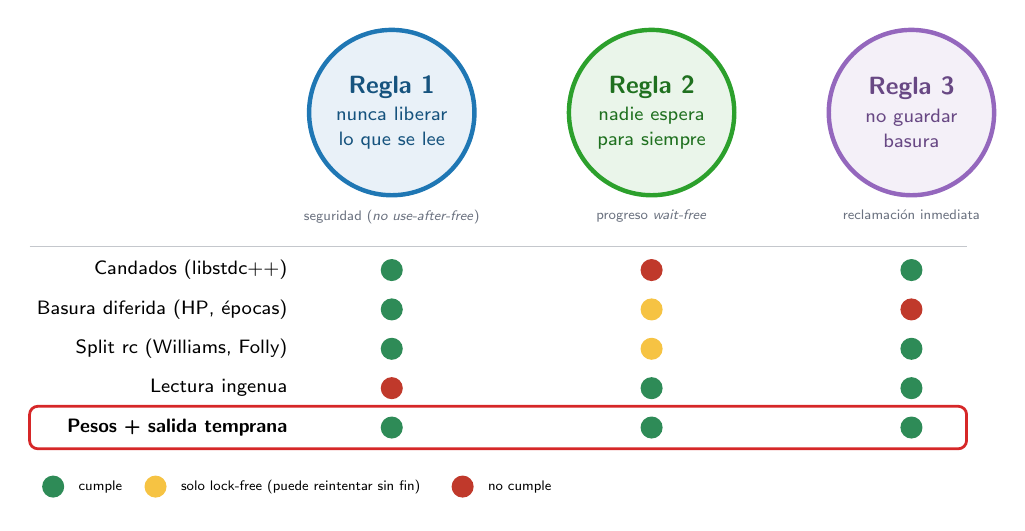
\begin{tikzpicture}[
    regla/.style={circle, draw=#1, line width=1.6pt, fill=#1!10, minimum size=2.1cm, align=center, font=\small\bfseries, text=#1!70!black},
    met/.style={font=\scriptsize, anchor=east},
    si/.style={circle, fill=verde, inner sep=0pt, minimum size=0.28cm},
    no/.style={circle, fill=acento, inner sep=0pt, minimum size=0.28cm},
    med/.style={circle, fill=amarillo, inner sep=0pt, minimum size=0.28cm}]
  % Las tres reglas
  \node[regla=cLib] (r1) at (0,0) {Regla 1\\[-1pt]\scriptsize\mdseries nunca liberar\\[-2pt]\scriptsize\mdseries lo que se lee};
  \node[regla=cWil] (r2) at (3.3,0) {Regla 2\\[-1pt]\scriptsize\mdseries nadie espera\\[-2pt]\scriptsize\mdseries para siempre};
  \node[regla=cAnd] (r3) at (6.6,0) {Regla 3\\[-1pt]\scriptsize\mdseries no guardar\\[-2pt]\scriptsize\mdseries basura};
  \node[font=\tiny, gris, below=1pt of r1] {seguridad (\emph{no use-after-free})};
  \node[font=\tiny, gris, below=1pt of r2] {progreso \emph{wait-free}};
  \node[font=\tiny, gris, below=1pt of r3] {reclamación inmediata};
  % Matriz de métodos
  \foreach \m/\y/\a/\b/\c in {
      Candados (libstdc++)/-2.0/si/no/si,
      Basura diferida (HP{,} épocas)/-2.5/si/med/no,
      Split rc (Williams{,} Folly)/-3.0/si/med/si,
      Lectura ingenua/-3.5/no/si/si,
      \textbf{Pesos + salida temprana}/-4.0/si/si/si} {
    \node[met] at (-1.2,\y) {\m};
    \node[\a] at (0,\y) {}; \node[\b] at (3.3,\y) {}; \node[\c] at (6.6,\y) {};
  }
  \draw[gris!40] (-4.6,-1.7) -- (7.3,-1.7);
  \draw[rounded corners=3pt, draw=cOur, line width=1pt] (-4.6,-4.27) rectangle (7.3,-3.73);
  % leyenda
  \node[si] at (-4.3,-4.75) {}; \node[font=\tiny, anchor=west] at (-4.1,-4.75) {cumple};
  \node[med] at (-3.0,-4.75) {}; \node[font=\tiny, anchor=west] at (-2.8,-4.75) {solo lock-free (puede reintentar sin fin)};
  \node[no] at (0.9,-4.75) {}; \node[font=\tiny, anchor=west] at (1.1,-4.75) {no cumple};
\end{tikzpicture}
\end{document}
